\chapter{پیچیدگی زمانی}

\index{پیچیدگی زمانی}

کارایی الگوریتم‌ها در برنامه‌نویسی رقابتی بسیار مهم است.
معمولاً طراحی الگوریتمی که مسئله را کند حل کند آسان است،
اما چالش واقعی، ابداع الگوریتمی سریع است.
اگر الگوریتم بیش از حد کند باشد، تنها بخشی از امتیاز یا هیچ امتیازی دریافت نخواهد کرد.

\key{پیچیدگی زمانی} یک الگوریتم تخمین می‌زند که الگوریتم برای یک ورودی مشخص، چه مقدار زمان مصرف خواهد کرد.
ایده اصلی این است که کارایی به عنوان تابعی نشان داده شود که پارامتر آن، اندازه ورودی است.
با محاسبه پیچیدگی زمانی، می‌توان بدون پیاده‌سازی متوجه شد آیا الگوریتم به اندازه کافی سریع است یا خیر.

\section{قواعد محاسبه}

پیچیدگی زمانی یک الگوریتم با نماد $O(\cdots)$ نشان داده می‌شود
که در آن سه نقطه نشان‌دهنده یک تابع است.
معمولاً متغیر $n$ بیانگر اندازه ورودی است.
برای مثال، اگر ورودی یک آرایه از اعداد باشد،
$n$ اندازه آرایه خواهد بود،
و اگر ورودی یک رشته باشد،
$n$ طول رشته خواهد بود.

\subsubsection*{حلقه‌ها}

دلیل رایج برای کند بودن یک الگوریتم این است که شامل حلقه‌های متعددی است که ورودی را پیمایش می‌کنند.
هرچه الگوریتم شامل حلقه‌های تودرتوی بیشتری باشد، کندتر است.
اگر $k$ حلقه تودرتو وجود داشته باشد، پیچیدگی زمانی $O(n^k)$ است.

برای مثال، پیچیدگی زمانی کد زیر $O(n)$ است:
\begin{lstlisting}
for (int i = 1; i <= n; i++) {
    // code
}
\end{lstlisting}

و پیچیدگی زمانی کد زیر $O(n^2)$ است:
\begin{lstlisting}
for (int i = 1; i <= n; i++) {
    for (int j = 1; j <= n; j++) {
        // code
    }
}
\end{lstlisting}

\subsubsection*{مرتبه بزرگی}

پیچیدگی زمانی تعداد دقیق دفعات اجرای کد درون حلقه را بیان نمی‌کند،
بلکه تنها مرتبه بزرگی را نشان می‌دهد.
در مثال‌های زیر، کد درون حلقه به ترتیب $3n$، $n+5$ و $\lceil n/2 \rceil$ بار اجرا می‌شود،
اما پیچیدگی زمانی هر کد $O(n)$ است.

\begin{lstlisting}
for (int i = 1; i <= 3*n; i++) {
    // code
}
\end{lstlisting}

\begin{lstlisting}
for (int i = 1; i <= n+5; i++) {
    // code
}
\end{lstlisting}

\begin{lstlisting}
for (int i = 1; i <= n; i += 2) {
    // code
}
\end{lstlisting}

به عنوان مثالی دیگر،
پیچیدگی زمانی کد زیر $O(n^2)$ است:

\begin{lstlisting}
for (int i = 1; i <= n; i++) {
    for (int j = i+1; j <= n; j++) {
        // code
    }
}
\end{lstlisting}

\subsubsection*{مراحل}

اگر الگوریتم از مراحل متوالی تشکیل شده باشد،
پیچیدگی زمانی کل برابر با بیشترین پیچیدگی زمانی در میان تک‌تک مراحل است.
دلیل این امر این است که کندترین مرحله معمولاً گلوگاه کد محسوب می‌شود.

برای مثال، کد زیر از سه مرحله با پیچیدگی‌های زمانی
$O(n)$، $O(n^2)$ و $O(n)$ تشکیل شده است.
بنابراین، پیچیدگی زمانی کل $O(n^2)$ است.

\begin{lstlisting}
for (int i = 1; i <= n; i++) {
    // code
}
for (int i = 1; i <= n; i++) {
    for (int j = 1; j <= n; j++) {
        // code
    }
}
for (int i = 1; i <= n; i++) {
    // code
}
\end{lstlisting}

\subsubsection*{چند متغیر}

گاهی پیچیدگی زمانی به چندین عامل بستگی دارد.
در این حالت، فرمول پیچیدگی زمانی شامل چند متغیر است.

برای نمونه، پیچیدگی زمانی کد زیر $O(nm)$ است:

\begin{lstlisting}
for (int i = 1; i <= n; i++) {
    for (int j = 1; j <= m; j++) {
        // code
    }
}
\end{lstlisting}

\subsubsection*{بازگشت}

پیچیدگی زمانی تابع بازگشتی به تعداد دفعات فراخوانی تابع و پیچیدگی زمانی یک فراخوانی بستگی دارد.
پیچیدگی زمانی کل برابر حاصل‌ضرب این مقادیر است.

برای نمونه، تابع زیر را در نظر بگیرید:
\begin{lstlisting}
void f(int n) {
    if (n == 1) return;
    f(n-1);
}
\end{lstlisting}
فراخوانی $\texttt{f}(n)$ موجب $n$ بار فراخوانی تابع می‌شود و پیچیدگی زمانی هر فراخوانی $O(1)$ است.
بنابراین، پیچیدگی زمانی کل $O(n)$ است.

به عنوان نمونه‌ای دیگر، تابع زیر را در نظر بگیرید:
\begin{lstlisting}
void g(int n) {
    if (n == 1) return;
    g(n-1);
    g(n-1);
}
\end{lstlisting}
در این حالت هر فراخوانی تابع دو فراخوانی دیگر ایجاد می‌کند، مگر برای $n=1$.
بررسی می‌کنیم هنگام فراخوانی $g$ با پارامتر $n$ چه رخ می‌دهد.
جدول زیر فراخوانی‌های تابع ایجاد شده توسط این تک‌فراخوانی را نشان می‌دهد:
\begin{center}
\begin{tabular}{rr}
فراخوانی تابع & تعداد فراخوانی‌ها \\
\hline
$g(n)$ & 1 \\
$g(n-1)$ & 2 \\
$g(n-2)$ & 4 \\
$\cdots$ & $\cdots$ \\
$g(1)$ & $2^{n-1}$ \\
\end{tabular}
\end{center}
بر این اساس، پیچیدگی زمانی برابر است با:
\[1+2+4+\cdots+2^{n-1} = 2^n-1 = O(2^n).\]

\section{رده‌های پیچیدگی}

\index{complexity classes}

فهرست زیر شامل پیچیدگی‌های زمانی متداول در الگوریتم‌ها است:

\begin{description}
\item[$O(1)$]
\index{constant-time algorithm}
زمان اجرای الگوریتم \key{زمان ثابت} به اندازه ورودی بستگی ندارد.
یک الگوریتم زمان ثابت نوعی، فرمول مستقیمی است که پاسخ را محاسبه می‌کند.

\item[$O(\log n)$]
\index{logarithmic algorithm}
یک الگوریتم \key{لگاریتمی} معمولاً اندازه ورودی را در هر گام نصف می‌کند.
زمان اجرای چنین الگوریتمی لگاریتمی است، زیرا $\log_2 n$ برابر با تعداد دفعاتی است که $n$ باید بر ۲ تقسیم شود تا به ۱ برسد.

\item[$O(\sqrt n)$]
یک \key{الگوریتم ریشه دوم} از $O(\log n)$ کندتر ولی از $O(n)$ سریع‌تر است.
ویژگی خاص ریشه دوم این است که $\sqrt n = n/\sqrt n$، بنابراین ریشه دوم $\sqrt n$ به نوعی در میانه ورودی قرار دارد.

\item[$O(n)$]
\index{linear algorithm}
یک الگوریتم \key{خطی} ورودی را به تعداد ثابتی پیمایش می‌کند.
این پیچیدگی زمانی اغلب بهترین حالت ممکن است، زیرا معمولاً دسترسی به هر عنصر ورودی حداقل یک بار پیش از اعلام پاسخ ضروری است.

\item[$O(n \log n)$]
این پیچیدگی زمانی اغلب نشان می‌دهد که الگوریتم ورودی را مرتب‌سازی می‌کند، زیرا پیچیدگی زمانی الگوریتم‌های کارآمد مرتب‌سازی $O(n \log n)$ است.
احتمال دیگر این است که الگوریتم از ساختمان داده‌ای استفاده می‌کند که در آن هر عملیات $O(\log n)$ زمان می‌برد.
\end{description}

\item[$O(n^2)$]
\index{quadratic algorithm}
یک الگوریتم \key{درجه‌دوم} اغلب شامل
دو حلقه تو‌در‌تو است.
بررسی تمام جفت‌های عناصر ورودی
در زمان $O(n^2)$ امکان‌پذیر است.

\item[$O(n^3)$]
\index{cubic algorithm}
یک الگوریتم \key{درجه‌سوم} اغلب شامل
سه حلقه تو‌در‌تو است.
بررسی تمام سه‌تایی‌های عناصر ورودی
در زمان $O(n^3)$ امکان‌پذیر است.

\item[$O(2^n)$]
این پیچیدگی زمانی اغلب نشان می‌دهد که
الگوریتم روی تمام زیرمجموعه‌های عناصر ورودی پیمایش می‌کند.
برای نمونه، زیرمجموعه‌های $\{1,2,3\}$ عبارتند از
$\emptyset$، $\{1\}$، $\{2\}$، $\{3\}$، $\{1,2\}$،
$\{1,3\}$، $\{2,3\}$ و $\{1,2,3\}$.

\item[$O(n!)$]
این پیچیدگی زمانی اغلب نشان می‌دهد که
الگوریتم روی تمام جایگشت‌های عناصر ورودی پیمایش می‌کند.
برای نمونه، جایگشت‌های $\{1,2,3\}$ عبارتند از
$(1,2,3)$، $(1,3,2)$، $(2,1,3)$، $(2,3,1)$،
$(3,1,2)$ و $(3,2,1)$.

\end{description}

\index{polynomial algorithm}
یک الگوریتم \key{چندجمله‌ای} است
اگر پیچیدگی زمانی آن حداکثر $O(n^k)$ باشد
که در آن $k$ یک مقدار ثابت است.
تمام پیچیدگی‌های زمانی بالا به جز
$O(2^n)$ و $O(n!)$ چندجمله‌ای هستند.
در عمل، ثابت $k$ معمولاً کوچک است،
و بنابراین پیچیدگی زمانی چندجمله‌ای
تقریباً به این معناست که الگوریتم \emph{کارآمد} است.

\index{NP-hard problem}

بیشتر الگوریتم‌های این کتاب چندجمله‌ای هستند.
با این حال، مسائل مهم زیادی وجود دارند که
هیچ الگوریتم چندجمله‌ای برای آن‌ها شناخته نشده است؛ به این معنی که
هیچ‌کس راه حل کارآمدی برای آن‌ها نمی‌داند.
مسائل \key{NP-سخت} دسته مهمی از مسائل هستند
که هیچ الگوریتم چندجمله‌ای برای آن‌ها شناخته نشده است\footnote{یک کتاب کلاسیک در این زمینه، کتاب
\emph{Computers and Intractability: A Guide to the Theory of NP-Completeness} اثر M. R. Garey و D. S. Johnson است \cite{gar79}.}.

\section{تخمین کارایی}

با محاسبه پیچیدگی زمانی یک الگوریتم،
می‌توان پیش از پیاده‌سازی بررسی کرد
که آیا الگوریتم برای حل مسئله به اندازه کافی کارآمد است یا خیر.
نقطه شروع تخمین‌ها این واقعیت است که
یک رایانه مدرن می‌تواند چند صد میلیون عملیات را در یک ثانیه انجام دهد.

برای نمونه، فرض کنید محدودیت زمانی یک مسئله
یک ثانیه و اندازه ورودی $n=10^5$ است.
اگر پیچیدگی زمانی $O(n^2)$ باشد،
الگوریتم حدود $(10^5)^2=10^{10}$ عملیات انجام خواهد داد.
این کار حداقل به چند ده ثانیه زمان نیاز دارد،
بنابراین الگوریتم برای حل مسئله بیش از حد کُند به نظر می‌رسد.

از سوی دیگر، با توجه به اندازه ورودی،
می‌توان پیچیدگی زمانی مورد نیاز الگوریتم حل‌کننده مسئله را
\emph{حدس} زد.
جدول زیر شامل چند تخمین کاربردی
با فرض محدودیت زمانی یک ثانیه است.

\begin{center}
\begin{tabular}{ll}
اندازه ورودی & پیچیدگی زمانی مورد نیاز \\
\hline
$n \le 10$ & $O(n!)$ \\
$n \le 20$ & $O(2^n)$ \\
$n \le 500$ & $O(n^3)$ \\
$n \le 5000$ & $O(n^2)$ \\
$n \le 10^6$ & $O(n \log n)$ یا $O(n)$ \\
$n$ بزرگ است & $O(1)$ یا $O(\log n)$ \\
\end{tabular}
\end{center}

به عنوان مثال، اگر اندازه ورودی $n=10^5$ باشد،
احتمالاً انتظار می‌رود که پیچیدگی زمانی
الگوریتم $O(n)$ یا $O(n \log n)$ باشد.
این اطلاعات طراحی الگوریتم را ساده‌تر می‌کند،
زیرا روش‌هایی را که منجر به الگوریتمی
با پیچیدگی زمانی بدتر می‌شوند کنار می‌گذارد.

\index{constant factor}

با این حال، باید به یاد داشت که
پیچیدگی زمانی تنها برآوردی از کارایی است،
زیرا \emph{ضرایب ثابت} را پنهان می‌کند.
برای نمونه، الگوریتمی با زمان اجرای $O(n)$
ممکن است $n/2$ یا $5n$ عملیات انجام دهد.
این موضوع اثر مهمی بر زمان اجرای واقعی
الگوریتم دارد.

\section{بیشینه مجموع زیرآرایه}

\index{maximum subarray sum}

اغلب چندین الگوریتم با پیچیدگی‌های زمانی
متفاوت برای حل یک مسئله وجود دارد.
این بخش مسئله‌ای کلاسیک را بررسی می‌کند که
یک راه حل مستقیم با زمان اجرای $O(n^3)$ دارد.
با این وجود، با طراحی الگوریتمی بهتر می‌توان
مسئله را در زمان $O(n^2)$ و حتی $O(n)$ حل کرد.

به ازای یک آرایه شامل $n$ عدد،
هدف محاسبه \key{بیشینه مجموع زیرآرایه} است؛ یعنی
بزرگ‌ترین مجموع ممکن از دنباله‌ای از مقادیر متوالی
در آرایه\footnote{کتاب \emph{Programming Pearls} نوشته J. Bentley \cite{ben86} این مسئله را معروف کرد.}.
این مسئله زمانی جالب می‌شود که مقادیر منفی
در آرایه وجود داشته باشند.
به عنوان مثال، در آرایه
\begin{center}
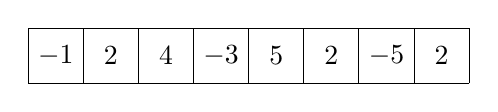
\begin{tikzpicture}[scale=0.7]
\draw (0,0) grid (8,1);

\node at (0.5,0.5) {$-1$};
\node at (1.5,0.5) {$2$};
\node at (2.5,0.5) {$4$};
\node at (3.5,0.5) {$-3$};
\node at (4.5,0.5) {$5$};
\node at (5.5,0.5) {$2$};
\node at (6.5,0.5) {$-5$};
\node at (7.5,0.5) {$2$};
\end{tikzpicture}
\end{center}
\begin{samepage}
زیرآرایه زیر بیشینه مجموع $10$ را تولید می‌کند:
\begin{center}
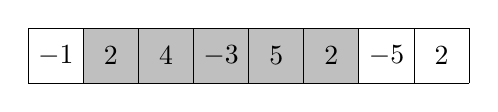
\begin{tikzpicture}[scale=0.7]
\fill[color=lightgray] (1,0) rectangle (6,1);
\draw (0,0) grid (8,1);

\node at (0.5,0.5) {$-1$};
\node at (1.5,0.5) {$2$};
\node at (2.5,0.5) {$4$};
\node at (3.5,0.5) {$-3$};
\node at (4.5,0.5) {$5$};
\node at (5.5,0.5) {$2$};
\node at (6.5,0.5) {$-5$};
\node at (7.5,0.5) {$2$};
\end{tikzpicture}
\end{center}
\end{samepage}

فرض می‌کنیم زیرآرایه خالی مجاز است،
بنابراین بیشینه مجموع زیرآرایه همیشه حداقل $0$ است.

\subsubsection{الگوریتم ۱}

یک روش مستقیم برای حل مسئله،
بررسی تمام زیرآرایه‌های ممکن،
محاسبه مجموع مقادیر هر زیرآرایه و نگهداری
بیشینه مجموع است.
کد زیر این الگوریتم را پیاده‌سازی می‌کند:

\begin{lstlisting}
int best = 0;
for (int a = 0; a < n; a++) {
    for (int b = a; b < n; b++) {
        int sum = 0;
        for (int k = a; k <= b; k++) {
            sum += array[k];
        }
        best = max(best,sum);
    }
}
cout << best << "\n";
\end{lstlisting}

متغیرهای \texttt{a} و \texttt{b} اندیس‌های ابتدا و
انتهای زیرآرایه را مشخص می‌کنند،
و مجموع مقادیر در متغیر \texttt{sum} محاسبه می‌شود.
متغیر \texttt{best} شامل بیشینه مجموع یافت‌شده در طول جستجو است.

پیچیدگی زمانی الگوریتم $O(n^3)$ است، زیرا از سه حلقه تو‌در‌تو تشکیل شده که ورودی را پیمایش می‌کنند.

\subsubsection{الگوریتم ۲}

بهینه‌تر کردن الگوریتم ۱ با حذف یک حلقه آسان است. این کار با محاسبه مجموع هم‌زمان با حرکت انتهای راست زیرآرایه ممکن می‌شود. نتیجه، کد زیر است:

\begin{lstlisting}
int best = 0;
for (int a = 0; a < n; a++) {
    int sum = 0;
    for (int b = a; b < n; b++) {
        sum += array[b];
        best = max(best,sum);
    }
}
cout << best << "\n";
\end{lstlisting}
پس از این تغییر، پیچیدگی زمانی $O(n^2)$ می‌شود.

\subsubsection{الگوریتم ۳}

به شکلی شگفت‌آور، حل این مسئله در زمان $O(n)$ ممکن است\footnote{در \cite{ben86}، این الگوریتم زمان‌خطی به جی. بی. کادین نسبت داده شده و الگوریتم گاهی \index{Kadane's algorithm} \key{الگوریتم کادین} نامیده می‌شود.}؛ یعنی فقط یک حلقه کافی است. ایده این است که برای هر جایگاه آرایه، بیشینه مجموع زیرآرایه‌ای محاسبه شود که در آن جایگاه پایان می‌یابد. پس از آن، پاسخ مسئله، بیشینه این مجموع‌ها خواهد بود.

زیرمسئله یافتن زیرآرایه با بیشینه مجموع را در نظر بگیرید که در جایگاه $k$ پایان می‌یابد. دو حالت وجود دارد:
\begin{enumerate}
\item زیرآرایه تنها شامل عنصر در جایگاه $k$ است.
\item زیرآرایه از یک زیرآرایه تشکیل شده که در جایگاه $k-1$ پایان می‌یابد و به دنبال آن عنصر در جایگاه $k$ می‌آید.
\end{enumerate}

در حالت دوم، از آنجا که به دنبال زیرآرایه‌ای با بیشینه مجموع هستیم، زیرآرایه‌ای که در جایگاه $k-1$ پایان می‌یابد نیز باید بیشینه مجموع را داشته باشد. بنابراین، می‌توان مسئله را با محاسبه بیشینه مجموع زیرآرایه برای هر جایگاه پایانی از چپ به راست، به صورت کارآمد حل کرد.

کد زیر الگوریتم را پیاده‌سازی می‌کند:
\begin{lstlisting}
int best = 0, sum = 0;
for (int k = 0; k < n; k++) {
    sum = max(array[k],sum+array[k]);
    best = max(best,sum);
}
cout << best << "\n";
\end{lstlisting}

الگوریتم تنها شامل یک حلقه است که ورودی را پیمایش می‌کند، بنابراین پیچیدگی زمانی $O(n)$ است. این مقدار، بهترین پیچیدگی زمانی ممکن نیز هست؛ زیرا هر الگوریتمی برای این مسئله باید تمام عناصر آرایه را دست‌کم یک بار بررسی کند.

\subsubsection{مقایسه کارایی}

بررسی میزان کارایی الگوریتم‌ها در عمل جالب است. جدول زیر زمان‌های اجرای الگوریتم‌های فوق را به ازای مقادیر مختلف $n$ روی یک رایانه امروزی نشان می‌دهد.

در هر آزمایش، ورودی به صورت تصادفی تولید شده است. زمان لازم برای خواندن ورودی اندازه‌گیری نشده است.

\begin{center}
\begin{tabular}{rrrr}
اندازه آرایه $n$ & الگوریتم ۱ & الگوریتم ۲ & الگوریتم ۳ \\
\hline
$10^2$ & $0.0$ s & $0.0$ s & $0.0$ s \\
$10^3$ & $0.1$ s & $0.0$ s & $0.0$ s \\
$10^4$ & > $10.0$ s & $0.1$ s & $0.0$ s \\
$10^5$ & > $10.0$ s & $5.3$ s & $0.0$ s \\
$10^6$ & > $10.0$ s & > $10.0$ s & $0.0$ s \\
$10^7$ & > $10.0$ s & > $10.0$ s & $0.0$ s \\
\end{tabular}
\end{center}

مقایسه نشان می‌دهد همه الگوریتم‌ها در اندازه‌های کوچک ورودی کارآمد هستند، اما ورودی‌های بزرگ‌تر تفاوت‌های چشمگیری در زمان اجرای الگوریتم‌ها آشکار می‌کنند.
الگوریتم ۱ در $n=10^4$ کند می‌شود و الگوریتم ۲ در $n=10^5$ کند می‌شود.
تنها الگوریتم ۳ می‌تواند حتی بزرگ‌ترین ورودی‌ها را نیز به صورت آنی پردازش کند.